% HMC Math dept HW template example
% v0.04 by Eric J. Malm, 10 Mar 2005
\documentclass[10pt,a4paper,boxed]{hmcpset}

% set 1-inch margins in the document
% \usepackage[margin=1in]{geometry}
\usepackage{enumerate}
\usepackage{todonotes}
%\usepackage{tikz}
%\usetikzlibrary{positioning}
\usepackage{subfig} % subfigures in figures.	
\usepackage{pgfplots}
\usepackage{amsmath}
\usepackage{amsfonts}
\usepackage{amssymb}

%% work around for subfig and asy environment
\makeatletter
\newsavebox{\sfe@box}
\newenvironment{subfloatenv}[2]{%
\def\sfe@caption{#1}%
\def\sfe@label{#2}%
\setbox\sfe@box\hbox\bgroup\color@setgroup}%
{\color@endgroup\egroup\subfloat[\sfe@caption]%
{\usebox{\sfe@box}\label{\sfe@label}}}
\makeatother

% include this if you want to import graphics files with /includegraphics
\usepackage{graphicx}

\renewcommand*{\familydefault}{\sfdefault}
\newcommand{\vect}[1]{\mathbf{#1}}


%\tikzset{node distance=2cm, inner/.style={draw,circle}, leaf/.style={draw,rectangle}}

\usepackage{hyperref}

% info for header block in upper right hand corner
\name{Lukas Gesing, Patrick Kaster}
\class{MA-INF 4201 - Artificial Life}
\assignment{Exercise Sheet 6}
% \duedate{09/03/2004}

\begin{document}


\begin{problem}[Assignment 37]
\end{problem}
We have:
\begin{align*}
	\log(N(t)) & = \log \left( a \frac{1}{s^\alpha} \right) \\
			   & = \log a + \log \left( \frac{1}{s^\alpha} \right) \\
			   & = \log (a) + \log (1) - \log \left( s^\alpha \right) \\
			   & = \log (a) + \log (1) - \alpha \cdot \log \left( s \right)
\end{align*}
So, apart from the logarithmic scaling, the expression is linear.
\begin{solution}
\end{solution}


\begin{problem}[Assignment 38]
\end{problem}
\begin{solution}
\begin{align*}
	N(k \cdot s) & = a \cdot \frac{1}{\left( k \cdot s \right)^\alpha} \\
			     & = a \cdot \frac{1}{k^\alpha} \cdot \frac{1}{s^\alpha} \\
			     & = \frac{1}{k^\alpha} \left( a \cdot \frac{1}{s^\alpha} \right)
\end{align*}
So, we have a proportionality constant of $\frac{1}{k^\alpha}$.
All power-law functions are scale invariant.
\end{solution}


\begin{problem}[Assignment 39]
\end{problem}
\begin{solution}
The primary problem is to the determine the corpus of the language/languages. Valid reserved words from the programming languages that compromise the corpus have to be distinguished from variable, etc., which might be terms from natural languages.

So one first has to know which programming languages to examine, in order to to derive keywords from their BNFs.

Subsequently the data might be gathered from large online software repositories.
\end{solution}


\begin{problem}[Assignment 40]
\end{problem}
\begin{solution}
\begin{description}
	\item[no guaranteed global minimum] The gradient decent method will converge to a local minimum, but no guarantee can be given that the minimum found is a global one. Thus, the method might not give the optimal solution.
	\item[result depends on initial conditions] Because of the above, the result will depend heavily on the initialization of the method, i.e. where on the surface of the objective function the decent is started.
	\item[not applicable to all objective functions] In order to do a decent and calculate a gradient, the objective function has to be continuous and differentiable, which makes the method non applicable to a whole range of functions. 
\end{description}
\end{solution}


\begin{problem}[Assignment 41]
\end{problem}
\begin{solution}
Both methods have in common, that the objective function doesn't have to be continuous nor differentiable. Instead both function pick a random position in search space.

The difference lies in the picking of a new random point in search space. While \emph{random search} samples the new point from the surface of a hypersphere that surrounds the current position, given a certain radius, the \emph{random optimization} draws a normally distributed vector and adds it to the current position.
\end{solution}


\begin{problem}[Assignment 42]
\end{problem}
\begin{solution}
For a starting concentration of $N_0 = 1 (100\%)$, we seek a factor $\lambda$, such that the function
\begin{align*}
	N(t) & = N_0 e^{-\lambda t}
\end{align*}
yields a value of $0.1 (10\%)$ after $t=42$.

To find the solution for $\lambda$ we solve the ODE
\begin{align*}
	\frac{dN}{dt} & = -\lambda N \Leftrightarrow \\
	\frac{dN}{N} & = -\lambda dt
\end{align*}
After integrating both sites we obtain:
\begin{align*}
	\ln \left( \frac{N}{N_0} \right) & = -\lambda t \Rightarrow \\
	 -\lambda & = \frac{\ln \left( \frac{N}{N_0} \right)}{t} 
\end{align*}
This gives the solution:
\begin{align*}
	 -\lambda & = \frac{\ln \left( 0.1 \right)}{42} \\
	 		  & = -0.054823454595096 
\end{align*}

As we easily verify:
\begin{align*}
	N(42) & = 1 \cdot e^{ -0.054823454595096 \cdot 42} \\
		  & = 0.1
\end{align*}

\end{solution}


\begin{problem}[Assignment 43]
\end{problem}
\begin{solution}
Without \emph{evaporation} the solution of the algorithm is static, i.e. a solution that is found once remains static, so that a dynamical change of the environment can't be accounted for.

Suppose a food source is found via an Ant-algorithm with \emph{evaporation}. After $n$ ants have transported back the food to the colony, the food source is depleted. Initially ants will follow the previous path to the food source, without finding more food. Thus, they won't return to the colony on the original path. The \emph{pheromone} trail will get weaker, until no ants returning from the colony will follow it anymore.

These ants will start searching for new food sources in random directions, increasing the probability to find a new food source.

Without \emph{evaporation} of the \emph{pheromone} trail the dynamic environmental change of food depletion doesn't lead to a new search phase of the algorithm.
\end{solution}

\begin{problem}[PA-C]
\end{problem}
\begin{solution}
The task has been implemented in python script \verb|PA-C.py| and has options \verb|-X| and \verb|-Y| for setting the starting conditions, as well as parameters \verb|-A| to \verb|-H|. Option \verb|-n| limits the number of iterations, option \verb|-m| gives an index position starting the mean calculation from. Parameter \verb|-S| determines the system of equations to calculate. It defaults to $0$ for the first system and $1$ for the second system. Options \verb|-G|, \verb|-H| are ignored for system $0$.

\emph{GNUPlot} is called from within the script after the calculation is done.

For the first equation set we used the following set of parameters:\\
./PA-C.py -X 0.03 -Y 0.02 -A 0.1 -B 0.1 -C 0.11 -D 0.02 -E -0.02 -F -2.2 -n 400 -m 200

For increasing parameter $a$ we observe that the mean grows, because variance increases, because oscillation becomes increasingly chaotic.

For the second equation set we used the following set of parameters:\\
./PA-C.py -X 0.03 -Y 0.02 -A 0.16 -B 0.1 -C 0.11 -D 0.02 -E -0.02 -F -2.2 -G 0.01 -H 0.01 -n 400 -m 200 -S 1

The major difference we observe is, that the system is coupled. Once the predator population begins oscillation, the prey population will follow shortly. Also the oscillation pattern is likewise.

	\begin{figure}[h]
		\centering
		\begin{subfloatenv}{output for first predator/prey system}{fig:system01}
			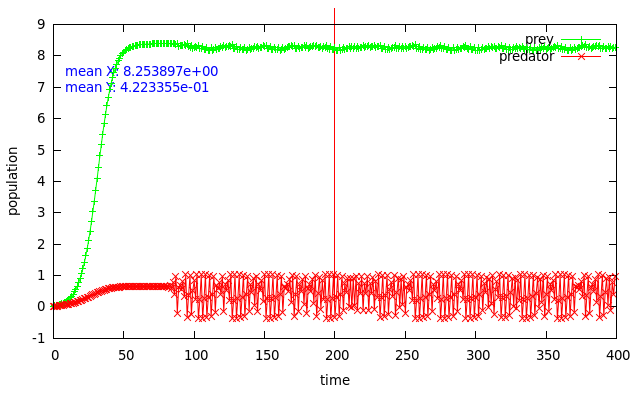
\includegraphics[width=0.4\textwidth]{img/PP01}
		\end{subfloatenv}
		\begin{subfloatenv}{output for second (coupled) predator/prey system}{fig:system02}
			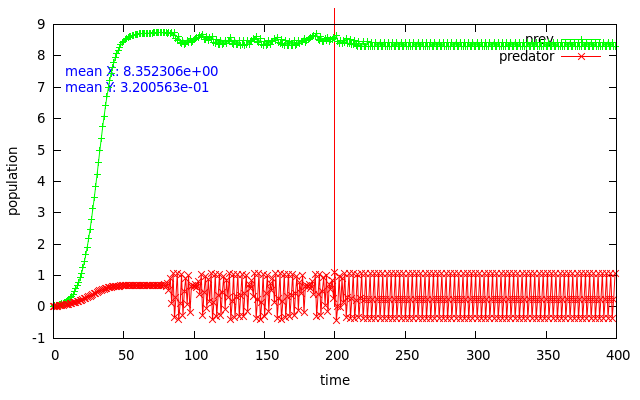
\includegraphics[width=0.4\textwidth]{img/PP02}
		\end{subfloatenv}
		%\caption{proof by induction over points on a circle}
			% das label muss immer nach der caption kommen, sonst gibt es Probleme bei der Referenzierung und Nummerierung.
		\label{fig:plots}
	\end{figure}
\end{solution}



\end{document}
